%%%%%%%%%%%%%%%%%%%%%%%%%%%%%%%%%%%%%%%%%
% fphw Assignment
% LaTeX Template
% Version 1.0 (27/04/2019)
%
% This template originates from:
% https://www.LaTeXTemplates.com
%
% Authors:
% Class by Felipe Portales-Oliva (f.portales.oliva@gmail.com) with template 
% content and modifications by Vel (vel@LaTeXTemplates.com)
%
% Template (this file) License:
% CC BY-NC-SA 3.0 (http://creativecommons.org/licenses/by-nc-sa/3.0/)
%
%%%%%%%%%%%%%%%%%%%%%%%%%%%%%%%%%%%%%%%%%

%----------------------------------------------------------------------------------------
%	PACKAGES AND OTHER DOCUMENT CONFIGURATIONS
%----------------------------------------------------------------------------------------

\documentclass[
	12pt, % Default font size, values between 10pt-12pt are allowed
	%letterpaper, % Uncomment for US letter paper size
	%spanish, % Uncomment for Spanish
]{fphw}

% Template-specific packages
\usepackage[utf8]{inputenc} % Required for inputting international characters
\usepackage[T1]{fontenc} % Output font encoding for international characters
\usepackage{mathpazo} % Use the Palatino font
\usepackage[dvipsnames]{xcolor}
\usepackage{graphicx} % Required for including images
\usepackage{amsmath}
\usepackage{booktabs} % Required for better horizontal rules in tables
\usepackage{listings} % Required for insertion of code
\usepackage{enumerate} % To modify the enumerate environment
\usepackage{ragged2e}
\usepackage{cancel}
\usepackage{MnSymbol,bbding,pifont}
\usepackage{lscape}
\usepackage{array}
\usepackage{float,graphicx}
\newcolumntype{M}{>{$}c<{$}}
%----------------------------------------------------------------------------------------
%	ASSIGNMENT INFORMATION
%----------------------------------------------------------------------------------------



\title{Project \#1} % Assignment title

\author{Luis Alberto Ballado Aradias} % Student name

\date{\today} % Due date

\institute{Centro de Investigación y de Estudios Avanzados del IPN \\ Unidad Tamaulipas} % Institute or school name

\class{Tecnologías Computacionales (Sep - Dec 2022)} % Course or class name

\professor{Dr. Edwin Aldana Bobadilla} % Professor or teacher in charge of the assignment

%----------------------------------------------------------------------------------------

\begin{document}

\maketitle % Output the assignment title, created automatically using the information in the custom commands above

%----------------------------------------------------------------------------------------
%	ASSIGNMENT CONTENT
%----------------------------------------------------------------------------------------
{\color{teal}
\dotfill
Polynomial Calculator
\dotfill}

\phantom{}\\
TALK A bit about lex and yacc

%\begin{figure}[H]
%  \centering
%  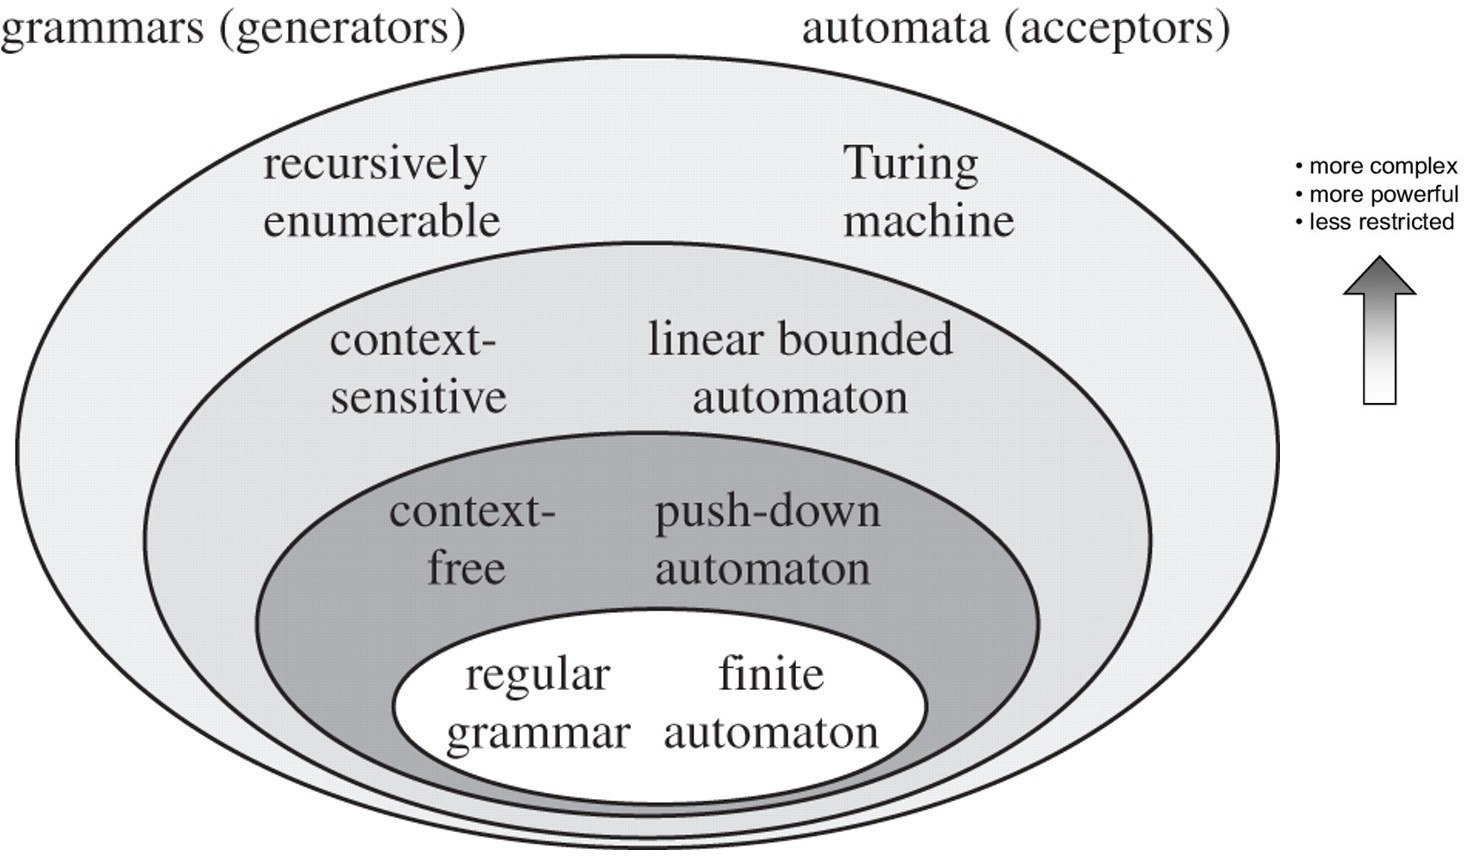
\includegraphics[scale=0.5]{images/chomsky_hierarchy.jpg}
%\end{figure}

The program is divided into 4 types:
\begin{enumerate}
\item Tokenization
\item Especificacion de tokens
\item Funciones de especificacion de tokens if apply  
\item Reglas de precedencia
\item Funcion de produccion
\end{enumerate}

\newpage
\section*{{\color{BlueViolet}Tokenization}}

Most restrictive of the set, they generate regular languages. They must have a single non-terminal on the left-hand-side and a right-hand-side consisting of a single terminal or single terminal followed by a single non-terminal.\\\\

\textbf{Example:}\\

Regex to define tokens such as identifiers, language keywords in programming languages. A coin vending machine that accepts only 1-Rupee, 2-Rupee and 5-Rupee coins has a regular language with only three words – 1, 2, 5.

\newpage
\section*{{\color{Apricot}Especificacion de tokens}}
%------------------------------------------------

Generate context-free languages, a category of immense interest to NLP practitioners. Here all rules take the form $A \implies \beta$, where A is a single non-terminal symbol and $\beta$ is a string of symbols.\\\\

\textbf{Example:}\\

Statement blocks in programming languages such as functions in parentheses, If-Else, for loops. In natural language, nouns and their plurals can be recognized through one Non Deterministic Finite Automaton (NFA), verbs and their different forms can be recognized through another NFA, and then combined. \\Singular (The girl runs home $\implies$ Girl + Runs). \\Plural (The girls run home $\implies$ Girls + Run)

%----------------------------------------------------------------------------------------

\newpage
\section*{{\color{Cerulean}Funciones de especificacion de tokens}}
%------------------------------------------------
The highest programmable level, they generate context-sensitive languages. They have rules of the form $\alpha A \beta \implies \alpha \gamma \beta$ with A as a non-terminal and $\alpha$, $\beta$, $\gamma$ as strings of terminals and non-terminals. Strings $\alpha$, $\beta$ may be empty, but $\gamma$ must be nonempty.\\\\

\textbf{Example:}\\

Though most language constructs in natural language are context-free, in some situations linear matching of tokens has to be done, such as - The square roots of 16, 9 and 4 are 4, 3 and 2, respectively. Here 16 is to be matched with 4, 9 is matched with 3, and 4 is matched with 2.

\newpage
\section*{{\color{RoyalPurple}Reglas de precedencia}}
%------------------------------------------------
Are too generic and unrestricted to describe the syntax of either programming or natural languages\\\\

\textbf{Example:}\\

A language with no restrictions is not conducive to communication or automation. Hence there are no common examples for this type. However, some mathematical seemingly unsolvable equations are expressed in this form.

%----------------------------------------------------------------------------------------

\newpage
\section*{{\color{RoyalPurple}Función de producción}}

Exercise: Create a regular expression to accept vehicle registration plates of Mexico State. There are three-letter series assigned \textbf{LGA-PEZ}

\begin{figure}[H]
  \centering
  
\includegraphics[scale=0.4]{images/placa_auto.png}
\end{figure}

\begin{verbatim}
/^[L-P]{1}[G-ZA-E]{1}[A-Z]{1}-\d{2}-\d{2}$/
\end{verbatim}

Explanation:\\



\end{document}
